\chapter{Описание алгоритмов}
\label{ch:chap1}

\section{K-RLE}

В контексте использования технологии беспроводной сенсорной сети
(WSN) для мониторинга окружающей среды двумя
основными элементарными функциями WSN являются сбор
и передача данных. Однако передача/прием данных
требует больших затрат энергии. Чтобы снизить энергопотребление, связанное с передачей, используется сжатие данных с помощью локальной обработки информации.

Рассмотрим новый алгоритм сжатия данных, основанный на кодировании длины выполнения (RLE), который называется K-RLE.

Идея, лежащая в основе этого нового алгоритма, заключается в следующем:
пусть $K$ - число, если элемент данных $d$, $d+K$ или $d-K$ встречается n раз подряд во входном потоке, мы заменяем эти n вхождений
одной парой $nd$ \cite{krle_article}.

\begin{figure}[ht]
    \centering
    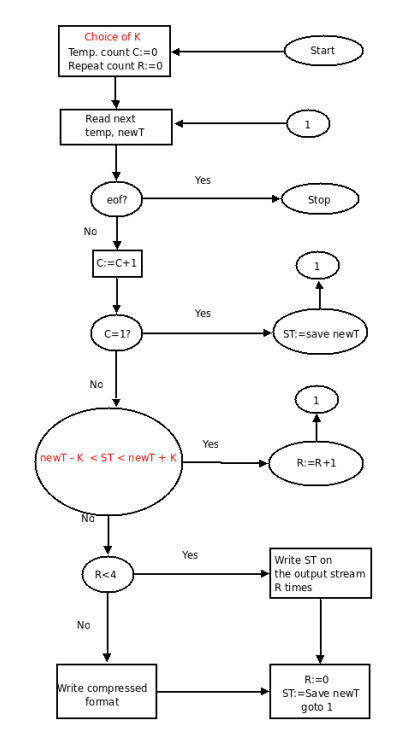
\includegraphics[width=0.5\textwidth]{krle_alg.png}
    \caption{K-RLE Алгоритм}
    \label{fig:krle_alg}
\end{figure}

\endinput